\documentclass[12pt,a4paper,fontset=none]{ctexart}

\usepackage[a4paper,margin=2.25cm]{geometry}
\usepackage{amsmath}
\usepackage{amssymb}
\usepackage{booktabs}
\usepackage{longtable}
\usepackage{array}
\usepackage{enumitem}
\usepackage{hyperref}
\usepackage{xcolor}
\usepackage{listings}
\usepackage{tikz}
\usetikzlibrary{arrows.meta,positioning,shapes.geometric,fit}

\setCJKmainfont{Microsoft JhengHei}
\setCJKsansfont{Microsoft JhengHei}
\setCJKmonofont{Microsoft JhengHei}

\hypersetup{
  colorlinks=true,
  linkcolor=blue!55!black,
  urlcolor=blue!55!black
}

\definecolor{dbgreen}{HTML}{0F766E}
\definecolor{dbgreenlight}{HTML}{E6F4F1}
\definecolor{dborange}{HTML}{D97706}
\definecolor{dbred}{HTML}{BE123C}
\definecolor{codebg}{HTML}{F8FAFC}

\lstdefinestyle{cmd}{
  basicstyle=\ttfamily\small,
  breaklines=true,
  frame=single,
  columns=fullflexible,
  backgroundcolor=\color{codebg},
  showstringspaces=false
}

\lstdefinestyle{sqlstyle}{
  basicstyle=\ttfamily\small,
  breaklines=true,
  frame=single,
  columns=fullflexible,
  backgroundcolor=\color{codebg},
  keywordstyle=\color{dbgreen}\bfseries,
  commentstyle=\color{gray},
  stringstyle=\color{dbred},
  showstringspaces=false
}

\lstdefinestyle{pystyle}{
  basicstyle=\ttfamily\small,
  breaklines=true,
  frame=single,
  columns=fullflexible,
  backgroundcolor=\color{codebg},
  keywordstyle=\color{blue!60!black}\bfseries,
  commentstyle=\color{gray},
  stringstyle=\color{dbred},
  showstringspaces=false
}

\setlist[itemize]{leftmargin=2em}
\setlist[enumerate]{leftmargin=2em}
\renewcommand{\arraystretch}{1.25}

\title{\textbf{shogiAI 資料庫系統與設計報告}\\
\large 系統架構、資料庫設計、ER 圖、Relational Model、建表 SQL、查詢、API 與 AI 訓練資料}
\author{shogiAI 專案}
\date{2026 年 6 月}

\begin{document}
\maketitle

\begin{abstract}
shogiAI 專案的資料庫系統以 MySQL 保存 CSA 將棋棋譜，將原始棋譜轉換為可查詢、可回放、可匯出訓練資料的關聯式資料模型。系統涵蓋資料蒐集、資料匯入、ER 設計、relational model、資料表設計、CREATE TABLE 程式碼、查詢功能、HTTP JSON API、前端棋譜瀏覽、AI 訓練資料匯出、資料品質、索引與維護操作。截至 2026-06-23 21:45，遠端 MySQL 資料庫包含 80,480 筆 \texttt{game\_records}、9,250,907 筆 \texttt{moves}、9,331,387 筆 \texttt{positions}、5,143 筆 \texttt{players} 與 2 筆 \texttt{users}，最晚資料寫入時間為 2026-06-23 04:56:24。
\end{abstract}

\tableofcontents
\newpage

\section{資料規模概況}

截至 2026-06-23 21:45，遠端 MySQL 資料庫的主要資料表規模如下。資料庫資料量大於 2026-06-16 模型訓練資料集，原因是爬蟲與 watcher 在訓練後仍持續匯入棋譜；模型訓練結果對應 2026-06-16 匯出的固定資料集，資料庫規模則反映目前累積狀態。

\begin{longtable}{p{0.40\textwidth}p{0.40\textwidth}}
\toprule
\textbf{資料表或項目} & \textbf{截至 2026-06-23 的數值}\\
\midrule
\endhead
\texttt{game\_records} & 80,480 筆\\
\texttt{moves} & 9,250,907 筆\\
\texttt{positions} & 9,331,387 筆\\
\texttt{players} & 5,143 筆\\
\texttt{users} & 2 筆\\
最早對局日期 & 1989-01-09\\
最晚對局日期 & 2026-05-19\\
最晚資料寫入時間 & 2026-06-23 04:56:24\\
\bottomrule
\end{longtable}

\begin{longtable}{p{0.40\textwidth}p{0.40\textwidth}}
\toprule
\textbf{棋局結果} & \textbf{\texttt{game\_records} 筆數}\\
\midrule
\endhead
\texttt{TORYO} & 79,728 筆\\
\texttt{SENNICHITE} & 751 筆\\
\texttt{DRAW} & 1 筆\\
\bottomrule
\end{longtable}

\section{專案目標}

shogiAI 的資料庫系統把原始 CSA 棋譜整理成可查詢、回放、訓練、驗證的資料資產。整體目標分成四個層次：

\begin{enumerate}
  \item \textbf{資料蒐集：} 從 shogidb2 網站取得棋局資料，轉成 CSA 檔案並保存。
  \item \textbf{資料管理：} 將 CSA 檔案匯入 MySQL，以正規化資料表保存棋手、對局、走法與局面。
  \item \textbf{資料服務：} 透過 HTTP JSON API 讓前端查詢棋局、回放任意手數、上傳新棋譜與取得資料庫統計。
  \item \textbf{AI 支援：} 由資料庫匯出 policy 訓練資料集，並從資料庫統計 opening book 供 AI 對弈使用。
\end{enumerate}

資料庫因此是整個專案的中樞。爬蟲、前端、後端、訓練程式與 AI 搜尋系統都圍繞同一份 MySQL 資料運作。

\section{資料庫系統目標}

shogiAI 的資料來源是 CSA 將棋棋譜。若只把每一盤棋保存成文字檔，雖然可以保留原始資料，但無法有效支援下列需求：

\begin{itemize}
  \item 依棋手、日期、賽事、開局或結果搜尋棋局。
  \item 在網頁上快速跳到任意手數並顯示棋盤。
  \item 上傳新的 CSA 棋譜並納入同一套資料系統。
  \item 匯出 AI 訓練資料，例如用目前局面預測下一手。
  \item 建立 opening book，統計同一局面下常見實戰手。
  \item 追蹤資料來源、避免重複匯入、檢查非法棋譜。
\end{itemize}

因此資料庫的核心任務不能是單純保存檔案，而要把一盤棋拆成可查詢、驗證、關聯、重複使用的資料結構。shogiAI 採用 MySQL 作為主要資料庫，並以 Python 程式負責建表、匯入、查詢與 API 回傳。

\section{整體系統架構}

專案由本地開發環境、遠端大數據主機、MySQL 主機與 GitHub 四個部分組成。

\begin{center}
\begin{tabular}{c}
shogidb2 網站 \\
$\downarrow$ \\
遠端大數據主機：\texttt{climbbug/CC.py} 爬取 CSA \\
$\downarrow$ \\
\texttt{watch\_csa\_import.py} 分批匯入 MySQL \\
$\downarrow$ \\
MySQL：\texttt{users}, \texttt{players}, \texttt{game\_records}, \texttt{moves}, \texttt{positions} \\
$\downarrow$ \\
\texttt{csa\_browser\_api.py} 提供 JSON API \\
$\downarrow$ \\
前端棋譜瀏覽器、AI 對弈、資料集匯出與模型訓練
\end{tabular}
\end{center}

本地與遠端的程式碼透過 GitHub \texttt{main} 分支同步。遠端負責長時間蒐集資料與訓練，本地負責開發、展示、文件撰寫與模型使用。

\section{遠端資料蒐集流程}

遠端爬蟲位於 \texttt{climbbug/CC.py}。它的目的，是從 shogidb2 網站取得公開棋局並轉成 CSA 格式。流程如下：

\begin{enumerate}
  \item 使用 \texttt{requests} 下載 shogidb2 的棋譜列表頁。
  \item 使用 \texttt{BeautifulSoup} 解析 HTML 中的棋局連結。
  \item 將棋局 URL 寫入 \texttt{game\_urls.txt}，避免重複掃描。
  \item 使用 Selenium 啟動 headless Chrome 開啟棋局頁面。
  \item 從 Chrome performance log 中讀取 WebSocket frame。
  \item 在 frame payload 中尋找包含 \texttt{moves} 與 \texttt{csa} 的棋局資料。
  \item 將棋手、賽事、地點、時間、戰型與每一步 CSA 走法組合成完整 CSA 文字。
  \item 寫入 \texttt{climbbug/data/gameN.csa}。
  \item 若抓取失敗，將 URL 寫入 \texttt{failed\_urls.txt}。
\end{enumerate}

這個設計同時使用靜態解析與瀏覽器自動化。列表頁可用 \texttt{requests} 和 HTML parser 快速取得；棋局內容則需要 Selenium，因為實際資料藏在瀏覽器接收到的動態訊息中。

\section{本地與遠端同步機制}

專案使用 GitHub 作為共同來源。同步腳本包含：

\begin{itemize}
  \item \texttt{sync\_repo.ps1}：本地 Windows 使用，負責 \texttt{git add}、\texttt{commit}、\texttt{pull --rebase}、\texttt{push}。
  \item \texttt{sync\_repo.sh}：Linux 環境使用，功能與 PowerShell 版本相同。
  \item \texttt{sync\_remote.sh}：遠端大數據主機使用，會先把 live crawler 目錄 \texttt{\$HOME/climbbug} 的資料複製進 repo 的 \texttt{climbbug/}，再提交推送，最後把 repo 內容同步回 live crawler 目錄。
\end{itemize}

這樣做的好處是遠端與本地不直接互相覆蓋，而是透過 Git 歷史保留每次資料與程式變更。如果兩邊改到同一檔案，Git rebase 會停下來要求解衝突，避免資料被靜默覆寫。

\section{設計需求分析}

\subsection{資料本身的特性}

一盤 CSA 棋譜同時包含多種資料：

\begin{itemize}
  \item 棋局層級資料：賽事名稱、地點、開局、結果、對局日期、原始檔名。
  \item 棋手層級資料：先手棋手、後手棋手、段位或稱號。
  \item 手順層級資料：第幾手、行棋方、原始 CSA 走法、標準 USI 走法、註解。
  \item 局面層級資料：每一手前後的 SFEN、是否王手、合法手數、局面 hash。
  \item 系統層級資料：上傳者、匯入者、建立時間、資料來源格式。
\end{itemize}

如果把這些資料全部放在同一張大表，會發生資料重複、更新困難、查詢混亂等問題。例如同一位棋手可能出現在上千盤棋中，如果每盤棋都重複寫棋手名稱，之後要修正名稱時就必須更新很多列。因此本專案把資料拆成五張主要資料表：

\begin{center}
\texttt{users}, \texttt{players}, \texttt{game\_records}, \texttt{moves}, \texttt{positions}
\end{center}

\subsection{系統功能需求}

shogiAI 的主要功能與資料庫需求如下：

\begin{longtable}{p{0.28\textwidth}p{0.64\textwidth}}
\toprule
\textbf{功能} & \textbf{資料庫需要支援的能力}\\
\midrule
\endhead
棋譜列表與搜尋 & 查詢 \texttt{game\_records}，並 join \texttt{players} 顯示先後手棋手。\\
任意手回放 & 以 \texttt{game\_id} 與 \texttt{move\_number} 直接取得 \texttt{positions.sfen}。\\
手順顯示 & 查詢同一 \texttt{game\_id} 下所有 \texttt{moves}，依手數排序。\\
CSA 上傳 & 新增 \texttt{game\_records}、\texttt{moves}、\texttt{positions}，並追蹤 \texttt{users}。\\
資料庫統計 & 計算棋局數、棋手數、走法數、局面數。\\
AI 訓練資料匯出 & join \texttt{positions} 與 \texttt{moves}，形成 $Position_t \rightarrow Move_{t+1}$。\\
Opening book & 以 \texttt{sfen\_hash} 或 SFEN 統計相同局面的下一手分布。\\
\bottomrule
\end{longtable}

\section{資料庫設計方法}

本專案採用關聯式資料庫 MySQL。設計時先拆出 CSA 棋譜中的主要實體：

\begin{itemize}
  \item 使用者或匯入者。
  \item 棋手。
  \item 一盤對局的 metadata。
  \item 每一步走法。
  \item 每一手後的局面。
\end{itemize}

因此資料庫拆成五張主要資料表：\texttt{users}、\texttt{players}、\texttt{game\_records}、\texttt{moves}、\texttt{positions}。這樣符合正規化精神：棋手名稱不重複存在每一步資料中，對局資料不混入局面資料，走法與局面也分開保存。

\subsection{走法與局面的核心關係}

本專案最重要的資料模型是：

\[
Position_t + Move_{t+1} \rightarrow Position_{t+1}
\]

\texttt{positions} 的第 0 筆代表初始局面，第 $t$ 筆代表走完第 $t$ 手後的局面；\texttt{moves} 的第 $t+1$ 筆代表從 \texttt{Position\_t} 出發的下一步。這個設計使系統可以：

\begin{itemize}
  \item 直接查詢任意手數，不必每次從第一手重播。
  \item 從 \texttt{positions} join \texttt{moves} 匯出「局面、下一手」訓練資料。
  \item 用 SFEN hash 統計重複局面或建立 opening book。
\end{itemize}

\section{ER 圖}

本專案的 ER 圖如下。中心是 \texttt{game\_records}，它代表一盤棋；一盤棋會連到兩位棋手，也會擁有多筆走法與多筆局面。若棋譜由系統匯入或使用者上傳，也會連到 \texttt{users}。

\begin{center}
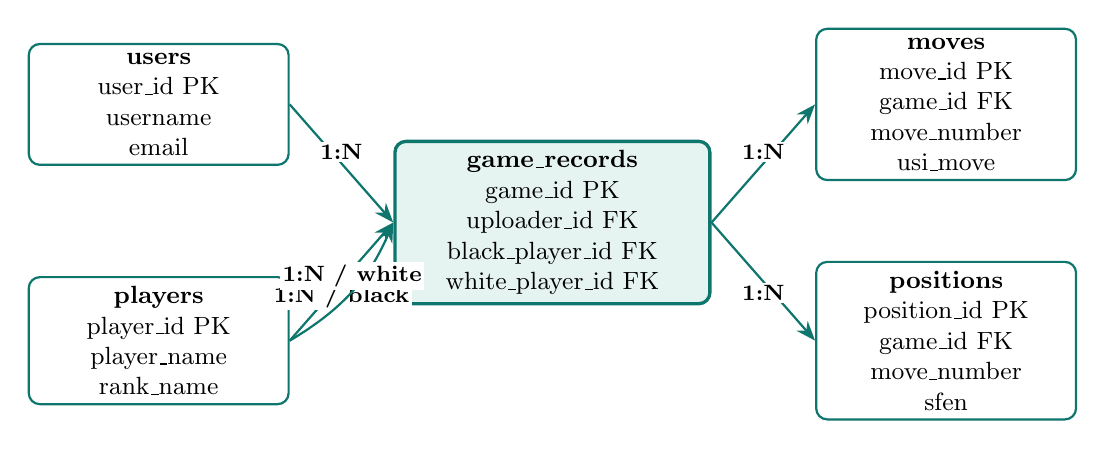
\begin{tikzpicture}[
  entity/.style={
    rectangle,
    rounded corners,
    draw=dbgreen,
    thick,
    fill=white,
    minimum width=3.3cm,
    minimum height=1.25cm,
    align=center,
    font=\small
  },
  core/.style={
    rectangle,
    rounded corners,
    draw=dbgreen,
    very thick,
    fill=dbgreenlight,
    minimum width=4.0cm,
    minimum height=1.6cm,
    align=center,
    font=\small
  },
  rel/.style={-{Stealth[length=2.5mm]}, thick, draw=dbgreen},
  label/.style={font=\footnotesize\bfseries, fill=white, inner sep=1pt}
]

\node[entity] (users) at (0,0) {
  \textbf{users}\\
  user\_id PK\\
  username\\
  email
};
\node[entity] (players) at (0,-3.0) {
  \textbf{players}\\
  player\_id PK\\
  player\_name\\
  rank\_name
};
\node[core] (games) at (5,-1.5) {
  \textbf{game\_records}\\
  game\_id PK\\
  uploader\_id FK\\
  black\_player\_id FK\\
  white\_player\_id FK
};
\node[entity] (moves) at (10,0) {
  \textbf{moves}\\
  move\_id PK\\
  game\_id FK\\
  move\_number\\
  usi\_move
};
\node[entity] (positions) at (10,-3.0) {
  \textbf{positions}\\
  position\_id PK\\
  game\_id FK\\
  move\_number\\
  sfen
};

\draw[rel] (users.east) -- node[label, above] {1:N} (games.west);
\draw[rel] (players.east) -- node[label, below] {1:N / black} (games.west);
\draw[rel] (players.east) to[bend right=18] node[label, above] {1:N / white} (games.west);
\draw[rel] (games.east) -- node[label, above] {1:N} (moves.west);
\draw[rel] (games.east) -- node[label, below] {1:N} (positions.west);

\end{tikzpicture}
\end{center}

\section{Relational Model}

Relational model 將 ER 圖轉成可在 MySQL 建立的關聯 schema。文字中的底線表示主鍵，並列出外鍵參照。

\subsection{\texttt{users}}

\[
\texttt{users}(
\underline{\texttt{user\_id}},
\texttt{username},
\texttt{email},
\texttt{password\_hash},
\texttt{role},
\texttt{created\_at}
)
\]

\begin{itemize}
  \item Primary Key: \texttt{user\_id}
  \item Unique: \texttt{email}
  \item 用途：記錄棋譜上傳者或匯入者，保留資料來源責任。
\end{itemize}

\subsection{\texttt{players}}

\[
\texttt{players}(
\underline{\texttt{player\_id}},
\texttt{player\_name},
\texttt{rank\_name},
\texttt{created\_at}
)
\]

\begin{itemize}
  \item Primary Key: \texttt{player\_id}
  \item 用途：保存棋手資料，避免棋手名稱在每一盤棋中重複出現。
\end{itemize}

\subsection{\texttt{game\_records}}

\[
\begin{aligned}
\texttt{game\_records}(
&\underline{\texttt{game\_id}},
\texttt{uploader\_id},
\texttt{black\_player\_id},
\texttt{white\_player\_id},\\
&\texttt{event\_name},
\texttt{site},
\texttt{opening},
\texttt{result},
\texttt{source\_format},\\
&\texttt{original\_file\_name},
\texttt{played\_at},
\texttt{created\_at})
\end{aligned}
\]

\begin{itemize}
  \item Primary Key: \texttt{game\_id}
  \item Foreign Key: \texttt{uploader\_id} references \texttt{users(user\_id)}
  \item Foreign Key: \texttt{black\_player\_id} references \texttt{players(player\_id)}
  \item Foreign Key: \texttt{white\_player\_id} references \texttt{players(player\_id)}
  \item 用途：保存一盤棋的 metadata，是整個 schema 的中心表。
\end{itemize}

\subsection{\texttt{moves}}

\[
\begin{aligned}
\texttt{moves}(
&\underline{\texttt{move\_id}},
\texttt{game\_id},
\texttt{move\_number},\\
&\texttt{side\_to\_move},
\texttt{original\_move},
\texttt{usi\_move},\\
&\texttt{move\_time},
\texttt{comment},
\texttt{created\_at})
\end{aligned}
\]

\begin{itemize}
  \item Primary Key: \texttt{move\_id}
  \item Foreign Key: \texttt{game\_id} references \texttt{game\_records(game\_id)}
  \item 用途：保存每一手走法，支援手順列表與棋譜回放。
\end{itemize}

\subsection{\texttt{positions}}

\[
\begin{aligned}
\texttt{positions}(
&\underline{\texttt{position\_id}},
\texttt{game\_id},
\texttt{move\_number},\\
&\texttt{side\_to\_move},
\texttt{sfen},
\texttt{sfen\_hash},\\
&\texttt{is\_check},
\texttt{legal\_moves\_count},
\texttt{created\_at})
\end{aligned}
\]

\begin{itemize}
  \item Primary Key: \texttt{position\_id}
  \item Foreign Key: \texttt{game\_id} references \texttt{game\_records(game\_id)}
  \item 用途：保存每一手對應局面，支援任意手查詢、AI 資料匯出與 opening book 統計。
\end{itemize}

\section{資料表設計}

\subsection{\texttt{users}}

\texttt{users} 保存系統使用者或匯入者，目前主要用於記錄資料來源與上傳者。

\begin{longtable}{p{0.28\textwidth}p{0.22\textwidth}p{0.40\textwidth}}
\toprule
\textbf{欄位} & \textbf{型別} & \textbf{用途}\\
\midrule
\endhead
\texttt{user\_id} & INT PK & 使用者主鍵，自動遞增。\\
\texttt{username} & VARCHAR & 使用者或匯入程式名稱。\\
\texttt{email} & VARCHAR UNIQUE & 可選信箱，也可作為匯入者識別。\\
\texttt{password\_hash} & VARCHAR & 預留登入功能。\\
\texttt{role} & VARCHAR & 權限角色，預設為 user。\\
\texttt{created\_at} & DATETIME & 建立時間。\\
\bottomrule
\end{longtable}

\subsection{\texttt{players}}

\texttt{players} 保存棋手資料，避免同一棋手在多盤棋中重複儲存。

\begin{longtable}{p{0.28\textwidth}p{0.22\textwidth}p{0.40\textwidth}}
\toprule
\textbf{欄位} & \textbf{型別} & \textbf{用途}\\
\midrule
\endhead
\texttt{player\_id} & INT PK & 棋手主鍵。\\
\texttt{player\_name} & VARCHAR & 棋手名稱。\\
\texttt{rank\_name} & VARCHAR & 段位或稱號。\\
\texttt{created\_at} & DATETIME & 建立時間。\\
\bottomrule
\end{longtable}

\subsection{\texttt{game\_records}}

\texttt{game\_records} 是對局主表，保存一盤棋的 metadata。

\begin{longtable}{p{0.30\textwidth}p{0.22\textwidth}p{0.38\textwidth}}
\toprule
\textbf{欄位} & \textbf{型別} & \textbf{用途}\\
\midrule
\endhead
\texttt{game\_id} & INT PK & 對局主鍵。\\
\texttt{uploader\_id} & INT FK & 匯入者，連到 \texttt{users}。\\
\texttt{black\_player\_id} & INT FK & 先手棋手，連到 \texttt{players}。\\
\texttt{white\_player\_id} & INT FK & 後手棋手，連到 \texttt{players}。\\
\texttt{event\_name} & VARCHAR & 賽事名稱。\\
\texttt{site} & VARCHAR & 對局地點。\\
\texttt{opening} & VARCHAR & 戰型或開局名稱。\\
\texttt{result} & VARCHAR & 結果，例如 TORYO、DRAW、SENNICHITE。\\
\texttt{source\_format} & VARCHAR & 來源格式，目前主要為 CSA。\\
\texttt{original\_file\_name} & VARCHAR & 原始檔名，用於追溯與去重。\\
\texttt{played\_at} & DATE & 對局日期。\\
\bottomrule
\end{longtable}

\subsection{\texttt{moves}}

\texttt{moves} 保存每一步棋。

\begin{longtable}{p{0.30\textwidth}p{0.22\textwidth}p{0.38\textwidth}}
\toprule
\textbf{欄位} & \textbf{型別} & \textbf{用途}\\
\midrule
\endhead
\texttt{move\_id} & INT PK & 走法主鍵。\\
\texttt{game\_id} & INT FK & 所屬對局。\\
\texttt{move\_number} & INT & 第幾手，從 1 開始。\\
\texttt{side\_to\_move} & ENUM & 下此手的一方，black 或 white。\\
\texttt{original\_move} & VARCHAR & 原始走法字串。\\
\texttt{usi\_move} & VARCHAR & 標準化 USI 走法。\\
\texttt{move\_time} & VARCHAR & 該手耗時。\\
\texttt{comment} & TEXT & 棋譜註解。\\
\bottomrule
\end{longtable}

\subsection{\texttt{positions}}

\texttt{positions} 保存局面。第 0 手是初始局面，第 $n$ 手代表走完第 $n$ 手後的盤面。

\begin{longtable}{p{0.30\textwidth}p{0.22\textwidth}p{0.38\textwidth}}
\toprule
\textbf{欄位} & \textbf{型別} & \textbf{用途}\\
\midrule
\endhead
\texttt{position\_id} & INT PK & 局面主鍵。\\
\texttt{game\_id} & INT FK & 所屬對局。\\
\texttt{move\_number} & INT & 此局面對應走完第幾手。\\
\texttt{side\_to\_move} & ENUM & 輪到哪一方行棋。\\
\texttt{sfen} & TEXT & 局面的 SFEN 表示。\\
\texttt{sfen\_hash} & CHAR(64) & SFEN 的 SHA-256 hash。\\
\texttt{is\_check} & BOOLEAN & 是否正在被王手。\\
\texttt{legal\_moves\_count} & INT & 此局面合法手數量。\\
\bottomrule
\end{longtable}

\section{如何 Create Database 與 Tables}

\subsection{手動建立資料庫}

在 MySQL 中可先建立專案資料庫。實際專案使用的資料庫名稱是 \texttt{DB11211213}。

\begin{lstlisting}[style=sqlstyle,language=SQL]
CREATE DATABASE IF NOT EXISTS DB11211213
  DEFAULT CHARACTER SET utf8mb4
  DEFAULT COLLATE utf8mb4_unicode_ci;

USE DB11211213;
\end{lstlisting}

\subsection{建立 \texttt{users}}

\begin{lstlisting}[style=sqlstyle,language=SQL]
CREATE TABLE IF NOT EXISTS users (
    user_id INT AUTO_INCREMENT PRIMARY KEY,
    username VARCHAR(100) NOT NULL,
    email VARCHAR(255) UNIQUE,
    password_hash VARCHAR(255),
    role VARCHAR(50) DEFAULT 'user',
    created_at DATETIME DEFAULT CURRENT_TIMESTAMP
) ENGINE=InnoDB DEFAULT CHARSET=utf8mb4;
\end{lstlisting}

\subsection{建立 \texttt{players}}

\begin{lstlisting}[style=sqlstyle,language=SQL]
CREATE TABLE IF NOT EXISTS players (
    player_id INT AUTO_INCREMENT PRIMARY KEY,
    player_name VARCHAR(100) NOT NULL,
    rank_name VARCHAR(50),
    created_at DATETIME DEFAULT CURRENT_TIMESTAMP
) ENGINE=InnoDB DEFAULT CHARSET=utf8mb4;
\end{lstlisting}

\subsection{建立 \texttt{game\_records}}

\begin{lstlisting}[style=sqlstyle,language=SQL]
CREATE TABLE IF NOT EXISTS game_records (
    game_id INT AUTO_INCREMENT PRIMARY KEY,
    uploader_id INT,
    black_player_id INT,
    white_player_id INT,
    event_name VARCHAR(255),
    site VARCHAR(255),
    opening VARCHAR(100),
    result VARCHAR(50),
    source_format VARCHAR(20),
    original_file_name VARCHAR(255),
    played_at DATE,
    created_at DATETIME DEFAULT CURRENT_TIMESTAMP,
    FOREIGN KEY (uploader_id) REFERENCES users(user_id),
    FOREIGN KEY (black_player_id) REFERENCES players(player_id),
    FOREIGN KEY (white_player_id) REFERENCES players(player_id)
) ENGINE=InnoDB DEFAULT CHARSET=utf8mb4;
\end{lstlisting}

\subsection{建立 \texttt{moves}}

\begin{lstlisting}[style=sqlstyle,language=SQL]
CREATE TABLE IF NOT EXISTS moves (
    move_id INT AUTO_INCREMENT PRIMARY KEY,
    game_id INT NOT NULL,
    move_number INT NOT NULL,
    side_to_move ENUM('black', 'white') NOT NULL,
    original_move VARCHAR(100),
    usi_move VARCHAR(20),
    move_time VARCHAR(50),
    comment TEXT,
    created_at DATETIME DEFAULT CURRENT_TIMESTAMP,
    FOREIGN KEY (game_id) REFERENCES game_records(game_id)
) ENGINE=InnoDB DEFAULT CHARSET=utf8mb4;
\end{lstlisting}

\subsection{建立 \texttt{positions}}

\begin{lstlisting}[style=sqlstyle,language=SQL]
CREATE TABLE IF NOT EXISTS positions (
    position_id INT AUTO_INCREMENT PRIMARY KEY,
    game_id INT NOT NULL,
    move_number INT NOT NULL,
    side_to_move ENUM('black', 'white') NOT NULL,
    sfen TEXT NOT NULL,
    sfen_hash CHAR(64),
    is_check BOOLEAN DEFAULT FALSE,
    legal_moves_count INT,
    created_at DATETIME DEFAULT CURRENT_TIMESTAMP,
    FOREIGN KEY (game_id) REFERENCES game_records(game_id)
) ENGINE=InnoDB DEFAULT CHARSET=utf8mb4;
\end{lstlisting}

\subsection{專案中的自動建表程式}

專案不是要求使用者手動執行每一段 SQL，而是在 \texttt{src/import\_csa\_to\_db.py} 中定義 \texttt{CREATE\_TABLES\_SQL}，並以 \texttt{ensure\_schema()} 自動建立資料表。

\begin{lstlisting}[style=pystyle,language=Python]
CREATE_TABLES_SQL = [
    """CREATE TABLE IF NOT EXISTS users (...)""",
    """CREATE TABLE IF NOT EXISTS players (...)""",
    """CREATE TABLE IF NOT EXISTS game_records (...)""",
    """CREATE TABLE IF NOT EXISTS moves (...)""",
    """CREATE TABLE IF NOT EXISTS positions (...)""",
]

def ensure_schema(cursor: Any) -> None:
    for sql in CREATE_TABLES_SQL:
        cursor.execute(sql)
\end{lstlisting}

匯入時若加上 \texttt{--create-tables} 參數，程式會先建立必要資料表：

\begin{lstlisting}[style=sqlstyle]
python src/import_csa_to_db.py ^
  --input climbbug/data ^
  --recursive ^
  --host 140.135.65.53 ^
  --port 3306 ^
  --user 11211213 ^
  --database DB11211213 ^
  --create-tables ^
  --skip-existing
\end{lstlisting}

\section{CSA 匯入 MySQL 流程}

匯入程式為 \texttt{src/import\_csa\_to\_db.py}。它負責把一個 CSA 檔案或整個資料夾中的 CSA 檔案匯入 MySQL。

\begin{enumerate}
  \item 掃描輸入路徑，支援單檔、資料夾與遞迴掃描。
  \item 使用 \texttt{cshogi.CSA.Parser} 解析 CSA。
  \item 解析棋手名稱、段位、賽事、地點、日期、戰型與結果。
  \item 建立或取得 \texttt{users} 與 \texttt{players} 資料。
  \item 建立 \texttt{game\_records} 對局。
  \item 用初始 SFEN 建立 \texttt{cshogi.Board}。
  \item 對每一步檢查 \texttt{board.is\_legal(move)}。
  \item 寫入 \texttt{moves}。
  \item 推進棋盤並寫入 \texttt{positions}。
  \item 每盤棋獨立 commit；錯誤時 rollback，避免半盤棋進入資料庫。
\end{enumerate}

匯入程式也支援 \texttt{--dry-run}、\texttt{--create-tables}、\texttt{--skip-existing}、\texttt{--max-games}、\\
\texttt{--pause-every} 等參數，使大量資料匯入可以分批進行並避免重複。

\section{資料匯入實例}

\subsection{新增棋局}

\begin{lstlisting}[style=pystyle,language=Python]
cursor.execute(
    """
    INSERT INTO game_records
        (
            uploader_id, black_player_id, white_player_id,
            event_name, site, opening, result, source_format,
            original_file_name, played_at
        )
    VALUES
        (%s, %s, %s, %s, %s, %s, %s, 'CSA', %s, %s)
    """,
    (
        uploader_id,
        black_player_id,
        white_player_id,
        info.get("EVENT"),
        info.get("SITE"),
        info.get("OPENING"),
        game_result(parser),
        file_key,
        parse_played_at(info.get("START_TIME")),
    ),
)
game_id = int(cursor.lastrowid)
\end{lstlisting}

這段程式的重點是先寫入一盤棋的 metadata，取得 \texttt{game\_id} 後，後面的 \texttt{moves} 與 \texttt{positions} 才能用外鍵連回這盤棋。

\subsection{新增手順}

\begin{lstlisting}[style=pystyle,language=Python]
cursor.executemany(
    """
    INSERT INTO moves
        (game_id, move_number, side_to_move,
         original_move, usi_move, move_time, comment)
    VALUES
        (%s, %s, %s, %s, %s, %s, %s)
    """,
    move_rows,
)
\end{lstlisting}

\texttt{move\_rows} 是程式解析 CSA 後產生的多筆走法資料。使用 \texttt{executemany()} 可以一次批次寫入多列，比逐列 \texttt{execute()} 更適合大量資料。

\subsection{新增局面}

\begin{lstlisting}[style=pystyle,language=Python]
cursor.executemany(
    """
    INSERT INTO positions
        (game_id, move_number, side_to_move,
         sfen, sfen_hash, is_check, legal_moves_count)
    VALUES
        (%s, %s, %s, %s, %s, %s, %s)
    """,
    position_rows,
)
\end{lstlisting}

\texttt{positions} 是本專案最重要的設計之一。一般棋譜只需要手順即可重播，但如果每次都從第一手重播到第 $n$ 手，前端跳手數與 AI 匯出資料會很慢。因此系統把每一手後的 SFEN 都存下來，讓任意手查詢變成直接查資料表。

\section{Position 與 Move 的對齊設計}

本專案最重要的資料庫設計是 \texttt{positions} 與 \texttt{moves} 的手數對齊。

\[
Position_t + Move_{t+1} \rightarrow Position_{t+1}
\]

\begin{itemize}
  \item \texttt{positions.move\_number = 0} 表示初始局面。
  \item \texttt{positions.move\_number = n} 表示走完第 $n$ 手後的局面。
  \item \texttt{moves.move\_number = 1} 表示第一手。
  \item \texttt{moves.move\_number = n} 表示第 $n$ 手走法。
\end{itemize}

因此若要匯出 AI 訓練資料，會使用：

\[
\texttt{positions.move\_number} + 1 = \texttt{moves.move\_number}
\]

這代表「用目前局面預測下一手」。這個設計同時支援四種功能：

\begin{enumerate}
  \item 前端棋譜回放：直接取第 $n$ 手局面。
  \item AI supervised learning：形成局面到下一手的訓練樣本。
  \item opening book：統計同一局面下常見下一手。
  \item 資料品質檢查：可驗證每一步走法是否能合法推進到下一局面。
\end{enumerate}

\section{查詢功能如何實現}

\subsection{棋局列表與搜尋}

前端呼叫 \texttt{GET /api/games} 時，後端會查詢 \texttt{game\_records}，並 join \texttt{players} 取得先手與後手棋手名稱。

\begin{lstlisting}[style=sqlstyle,language=SQL]
SELECT
    g.game_id,
    g.original_file_name,
    COALESCE(bp.player_name, 'black') AS black_player,
    COALESCE(wp.player_name, 'white') AS white_player,
    COALESCE(g.event_name, '') AS event_name,
    COALESCE(g.opening, '') AS opening,
    COALESCE(g.result, '') AS result,
    g.played_at,
    (
        SELECT COUNT(1)
        FROM moves m
        WHERE m.game_id = g.game_id
    ) AS move_count
FROM game_records g
LEFT JOIN players bp ON g.black_player_id = bp.player_id
LEFT JOIN players wp ON g.white_player_id = wp.player_id
WHERE ...
ORDER BY g.played_at DESC, g.game_id DESC
LIMIT ? OFFSET ?;
\end{lstlisting}

搜尋條件由 \texttt{build\_filters()} 組出，支援：

\begin{itemize}
  \item \texttt{event}: 依賽事名稱模糊查詢。
  \item \texttt{date\_from}: 起始日期。
  \item \texttt{date\_to}: 結束日期。
  \item \texttt{player}: 先手或後手棋手名稱。
  \item \texttt{opening}: 開局名稱。
\end{itemize}

\subsection{取得某盤棋第 n 手局面}

前端呼叫：

\begin{lstlisting}[style=sqlstyle]
GET /api/games/{game_id}?ply=n
\end{lstlisting}

後端會先確認手數範圍，再查詢 \texttt{positions}：

\begin{lstlisting}[style=sqlstyle,language=SQL]
SELECT move_number, side_to_move, sfen, is_check, legal_moves_count
FROM positions
WHERE game_id = %s AND move_number = %s
LIMIT 1;
\end{lstlisting}

同時也會撈出整盤手順，讓前端可以顯示 move list：

\begin{lstlisting}[style=sqlstyle,language=SQL]
SELECT move_number, side_to_move, original_move, usi_move, comment
FROM moves
WHERE game_id = %s
ORDER BY move_number;
\end{lstlisting}

這個功能之所以能有效率，是因為 \texttt{positions} 已經保存每個手數的 SFEN，不需要每次從頭重播棋局。

\subsection{資料庫統計}

\texttt{GET /api/db/stats} 會統計核心資料表：

\begin{lstlisting}[style=sqlstyle,language=SQL]
SELECT COUNT(1) AS count_value FROM game_records;
SELECT COUNT(1) AS count_value FROM players;
SELECT COUNT(1) AS count_value FROM moves;
SELECT COUNT(1) AS count_value FROM positions;
\end{lstlisting}

前端會把這些數字顯示成資料庫狀態，讓使用者知道目前資料規模。

\subsection{AI 訓練資料匯出查詢}

AI 訓練資料匯出使用 \texttt{positions} join \texttt{moves}：

\begin{lstlisting}[style=sqlstyle,language=SQL]
SELECT
    p.game_id,
    p.move_number,
    p.sfen,
    m.usi_move,
    p.side_to_move,
    g.result
FROM positions p
JOIN moves m
  ON m.game_id = p.game_id
 AND m.move_number = p.move_number + 1
JOIN game_records g
  ON g.game_id = p.game_id
ORDER BY p.game_id, p.move_number;
\end{lstlisting}

這個查詢把每一列轉成：

\[
\texttt{sfen} \rightarrow \texttt{usi\_move}
\]

接著 Python 會用 \texttt{cshogi.Board(sfen)} 還原棋盤，把 \texttt{usi\_move} 編碼成 policy label，最後存成 \texttt{.npz} 訓練資料。

\section{後端 API 設計}

後端位於 \texttt{src/csa\_browser\_api.py}，使用 Python 標準函式庫的 \texttt{ThreadingHTTPServer} 與 \texttt{BaseHTTPRequestHandler}。它同時支援 MySQL 資料來源與本機 CSA 檔案資料來源。

\begin{longtable}{p{0.34\textwidth}p{0.56\textwidth}}
\toprule
\textbf{API} & \textbf{功能}\\
\midrule
\endhead
\texttt{GET /api/games} & 查詢對局列表，支援事件、日期、棋手、開局等篩選。\\
\texttt{GET /api/games/<id>?ply=n} & 取得某盤棋第 $n$ 手局面，用於棋盤回放。\\
\texttt{GET /api/db/stats} & 回傳棋局、棋手、走法、局面與重複資料統計。\\
\texttt{POST /api/upload-csa} & 接收前端上傳的 CSA，保存到 \texttt{data/uploads} 並匯入 MySQL。\\
\texttt{POST /api/self-play/state} & 根據 USI 手順重播自我對弈狀態。\\
\texttt{POST /api/self-play/csa} & 將自我對弈手順輸出成 CSA 文字。\\
\texttt{POST /api/ai-play/state} & 回傳 AI 對弈目前盤面與 policy 候選手。\\
\texttt{POST /api/ai-play/move} & 讓 AI 搜尋並下一手。\\
\texttt{POST /api/policy/candidates} & 回傳目前局面的 policy 候選手。\\
\texttt{POST /api/model-match/step} & 執行模型互打一個 step。\\
\texttt{POST /api/model-match/run} & 執行多局模型互打。\\
\bottomrule
\end{longtable}


\section{API 功能與資料庫對應}

雖然本報告主軸是資料庫，但 API 是資料庫功能被前端使用的入口。下表整理每個 API 背後使用的資料表。

\begin{longtable}{p{0.32\textwidth}p{0.28\textwidth}p{0.32\textwidth}}
\toprule
\textbf{API} & \textbf{主要資料表} & \textbf{功能}\\
\midrule
\endhead
\texttt{GET /api/games} & \texttt{game\_records}, \texttt{players}, \texttt{moves} & 搜尋棋局、分頁、顯示棋手與手數。\\
\texttt{GET /api/games/<id>?ply=n} & \texttt{positions}, \texttt{moves}, \texttt{game\_records} & 取得第 $n$ 手棋盤與完整手順。\\
\texttt{GET /api/db/stats} & 所有核心表 & 顯示棋局數、棋手數、走法數、局面數。\\
\texttt{POST /api/upload-csa} & \texttt{users}, \texttt{game\_records}, \texttt{moves}, \texttt{positions} & 上傳 CSA 並匯入資料庫。\\
\texttt{POST /api/ai-play/move} & \texttt{positions}, opening book, model & AI 對弈時取得局面、候選手與搜尋結果。\\
\bottomrule
\end{longtable}

\section{前端棋譜瀏覽器}

前端位於 \texttt{web/index.html}、\texttt{web/app.js} 與 \texttt{web/styles.css}。它是一個原生 JavaScript 應用，透過 Fetch API 呼叫後端。

主要功能包含：

\begin{itemize}
  \item \textbf{棋譜列表：} 從 \texttt{/api/games} 載入對局，支援條件搜尋。
  \item \textbf{棋盤回放：} 使用 \texttt{/api/games/<id>?ply=n} 跳到任意手數。
  \item \textbf{資料庫統計：} 顯示目前 MySQL 中的資料量與重複群組。
  \item \textbf{CSA 上傳：} 前端用 multipart form 上傳，後端匯入 MySQL。
  \item \textbf{自我對弈：} 使用者可手動下棋並匯出 CSA。
  \item \textbf{AI 對弈：} 使用者與 AI 對弈，畫面顯示搜尋評分、深度、節點、PV 與 policy 候選手。
  \item \textbf{模型互打：} 選擇兩個 policy model，以相同搜尋框架互相對弈比較。
\end{itemize}

\section{資料庫設計如何支援各項功能}

\subsection{棋譜瀏覽}

棋譜瀏覽器需要三類資料：

\begin{itemize}
  \item 棋局列表：來自 \texttt{game\_records} 與 \texttt{players}。
  \item 棋盤局面：來自 \texttt{positions.sfen}。
  \item 手順列表：來自 \texttt{moves}。
\end{itemize}

因為 \texttt{positions} 保存每一手的 SFEN，前端可以在上一手、下一手、跳到最後一手之間快速切換。

\subsection{CSA 上傳}

上傳 CSA 後，後端會：

\begin{enumerate}
  \item 檢查副檔名與檔案大小。
  \item 保存到 \texttt{data/uploads}。
  \item 呼叫匯入程式。
  \item 若棋譜合法，新增 \texttt{game\_records}、\texttt{moves}、\texttt{positions}。
  \item 回傳新棋局的 \texttt{gameId}，前端切換到棋譜瀏覽畫面。
\end{enumerate}

\subsection{AI 訓練}

policy-only 模型需要大量：

\[
(\text{目前局面}, \text{下一手})
\]

資料庫的 \texttt{positions} 與 \texttt{moves} 正好提供這個結構。因此 AI 訓練不需要重新讀每個 CSA 檔案，可以直接從 MySQL 取出標準化後的資料。

\subsection{Opening Book}

Opening book 的概念是：如果同一個局面在實戰棋譜中出現很多次，就統計高手常下哪一手。資料庫中 \texttt{sfen} 與 \texttt{sfen\_hash} 讓系統能辨識相同局面，進而計算每個候選手的出現次數與比例。

\section{資料庫如何支援 AI}

資料庫對 AI 有三個用途。

\subsection{訓練資料匯出}

\texttt{src/export\_policy\_dataset.py} 從 MySQL 取出每個 \texttt{Position\_t} 與下一手 \texttt{Move\_{t+1}}：

\begin{lstlisting}[style=cmd]
SELECT p.game_id, p.move_number, p.sfen, m.usi_move, g.result
FROM positions p
JOIN moves m
  ON m.game_id = p.game_id
 AND m.move_number = p.move_number + 1
JOIN game_records g
  ON g.game_id = p.game_id
ORDER BY p.game_id, p.move_number;
\end{lstlisting}

匯出後會產生 \texttt{states}、\texttt{moves}、\texttt{game\_ids}、\texttt{meta} 等 NumPy arrays，供 policy network 訓練。

\subsection{Opening Book}

\texttt{OpeningBook.from\_mysql} 從 MySQL 統計前若干手中，同一 SFEN 的常見下一手。若某手出現次數達到門檻，AI 可在開局階段直接採用資料庫中的常見實戰走法。這能降低開局搜尋成本，也讓 AI 的開局更接近人類實戰資料。

\subsection{AI 對弈資料服務}

AI 對弈時，資料庫提供棋譜回放與訓練來源；模型提供 policy 候選手排序；傳統搜尋負責局面計算。系統已移除神經網路 value head，資料庫主要支援 policy 訓練與 opening book。

\section{資料品質與去重}

\subsection{合法手驗證}

資料品質最重要的步驟是合法性檢查。CSA 走法在寫入資料庫前會轉成 cshogi move，並以目前棋盤狀態檢查是否為合法手。若發現非法走法，該盤棋會 rollback，不會留下不完整資料。

\subsection{檔名去重}

\texttt{original\_file\_name} 可用於快速判斷同名 CSA 是否已經匯入。使用 \texttt{--skip-existing} 時，匯入程式會跳過已存在檔名。

\subsection{內容去重}

只靠檔名不夠，因為同一盤棋可能被重新命名。系統另外使用內容 key：

\[
SHA256(\text{initial SFEN} + \text{full USI move sequence})
\]

只要初始局面與完整走法序列相同，就視為同一盤棋。這能避免同一棋譜因檔名不同而重複匯入。

\section{資料品質與交易控制}

資料庫系統不只要能寫入資料，也要保證資料品質。

\subsection{合法性檢查}

匯入過程會用 \texttt{cshogi} 還原棋盤並檢查走法是否合法。如果某一步不合法，代表棋譜資料可能損壞或格式不正確，該盤棋不應寫入正式資料庫。

\subsection{重複資料處理}

系統使用兩種方式避免重複匯入：

\begin{itemize}
  \item \texttt{original\_file\_name}: 檢查同一檔名是否已匯入。
  \item content key: 以初始 SFEN 加完整 USI 手順產生 hash，即使檔名不同也能辨認同一盤棋。
\end{itemize}

\subsection{交易控制}

一盤棋匯入會同時寫入多張表。如果寫到一半失敗，資料庫可能留下沒有手順的棋局或沒有局面的棋局。因此匯入程式應該以 transaction 包住整盤棋的寫入：

\begin{itemize}
  \item 全部成功：commit。
  \item 任一步驟失敗：rollback。
\end{itemize}

這能保證資料庫不會留下半成品。


\section{效能與索引建議}

系統常見查詢包含依 \texttt{game\_id} 與 \texttt{move\_number} 查局面、依檔名去重、依日期或棋手搜尋對局、依 \texttt{sfen\_hash} 統計重複局面。建議索引如下：

\begin{lstlisting}[style=cmd]
CREATE INDEX idx_game_records_original_file_name
ON game_records(original_file_name);

CREATE INDEX idx_game_records_played_at
ON game_records(played_at);

CREATE INDEX idx_moves_game_number
ON moves(game_id, move_number);

CREATE INDEX idx_positions_game_number
ON positions(game_id, move_number);

CREATE INDEX idx_positions_sfen_hash
ON positions(sfen_hash);
\end{lstlisting}

\texttt{idx\_positions\_game\_number} 對前端回放最重要，因為每次跳手數都會用到。 \texttt{idx\_moves\_game\_number} 對資料集匯出最重要，因為匯出時需要把 position 與下一手 move 對齊。

\section{索引設計建議}

目前程式已能建立資料表與執行查詢。資料量已達 80,480 局與超過 933 萬筆局面資料，索引設計會直接影響前端回放、資料集匯出與 opening book 查詢速度。建議加入下列索引：

\begin{lstlisting}[style=sqlstyle,language=SQL]
CREATE INDEX idx_game_records_played_at
  ON game_records (played_at, game_id);

CREATE INDEX idx_players_name
  ON players (player_name);

CREATE INDEX idx_moves_game_number
  ON moves (game_id, move_number);

CREATE INDEX idx_positions_game_number
  ON positions (game_id, move_number);

CREATE INDEX idx_positions_sfen_hash
  ON positions (sfen_hash);
\end{lstlisting}

各索引用途如下：

\begin{longtable}{p{0.38\textwidth}p{0.52\textwidth}}
\toprule
\textbf{索引} & \textbf{用途}\\
\midrule
\endhead
\texttt{game\_records(played\_at, game\_id)} & 棋局列表依日期排序與分頁。\\
\texttt{players(player\_name)} & 棋手搜尋與 join。\\
\texttt{moves(game\_id, move\_number)} & 取得某盤棋全部手順。\\
\texttt{positions(game\_id, move\_number)} & 快速定位某盤棋第 $n$ 手局面。\\
\texttt{positions(sfen\_hash)} & 統計相同局面，支援 opening book。\\
\bottomrule
\end{longtable}

索引能提升讀取速度，但會增加寫入成本。因此不應該對所有欄位都建立索引，而是依照實際功能的高頻查詢建立。

\section{限制與未來改進}

目前系統仍有一些限制：

\begin{itemize}
  \item 匯出訓練資料時中途缺少細部進度列，資料量大時主要依程序狀態與 log 判斷進度。
  \item MySQL 匯入與訓練匯出可能同時發生，需要更完整的排程管理。
  \item 前端統計仍偏基本，可加入戰型分布、棋手分布、年份分布等分析。
  \item 資料庫 schema 可加入更多唯一約束與索引，以提高去重與查詢效能。
  \item 上傳功能目前適合內部展示，若要公開使用仍需登入、權限與檔案掃描。
\end{itemize}

\section{設計限制與改進方向}

\subsection{目前限制}

\begin{itemize}
  \item 建表 SQL 目前主要建立基本 foreign key，尚未在程式中建立所有建議索引。
  \item \texttt{players} 尚未對棋手名稱與段位建立唯一約束，因此同名不同寫法仍可能分裂。
  \item \texttt{positions.sfen} 使用 TEXT，若大量查詢完整 SFEN，應優先查 \texttt{sfen\_hash}。
  \item \texttt{users.password\_hash} 欄位目前保留，但完整登入權限系統尚未完善。
\end{itemize}

\subsection{未來可改進}

\begin{itemize}
  \item 加入 migration 工具，讓 schema 更新可以版本化。
  \item 補上索引建立腳本，特別是 \texttt{positions(game\_id, move\_number)}。
  \item 對棋手名稱建立清洗與合併規則，避免同一棋手被視為多人。
  \item 建立資料品質 dashboard，統計非法棋譜、重複棋譜與匯入錯誤。
  \item 強化 API 權限控管，限制上傳與刪除等高風險操作。
\end{itemize}

\section{常用操作指令}

\subsection{匯入 CSA 到 MySQL}

\begin{lstlisting}[style=cmd]
python src\import_csa_to_db.py ^
  --input data ^
  --recursive ^
  --create-tables ^
  --host 140.135.65.53 ^
  --port 3306 ^
  --user 11211213 ^
  --database DB11211213 ^
  --skip-existing
\end{lstlisting}

\subsection{啟動瀏覽器 API}

\begin{lstlisting}[style=cmd]
python src\csa_browser_api.py ^
  --source mysql ^
  --db-host 140.135.65.53 ^
  --db-port 3306 ^
  --db-user 11211213 ^
  --db-name DB11211213 ^
  --policy-model models\policy_model.pt ^
  --policy-order-ply 2 ^
  --opening-book-ply 30 ^
  --opening-book-min-count 2
\end{lstlisting}

\subsection{匯出 policy 訓練資料}

\begin{lstlisting}[style=cmd]
python src\export_policy_dataset.py ^
  --output out\policy_dataset.npz ^
  --host 140.135.65.53 ^
  --port 3306 ^
  --user 11211213 ^
  --database DB11211213
\end{lstlisting}

\section{系統層結論}

shogiAI 的資料庫系統將 CSA 棋譜轉換成可查詢、回放、訓練的關聯式資料。遠端爬蟲負責持續蒐集棋譜，後端 API 負責把資料轉成前端與 AI 可用的 JSON，前端提供使用者互動介面是串接資料蒐集、棋譜管理、AI 訓練與 AI 對弈的核心基礎。截至 2026-06-23，資料庫已累積 80,480 局與超過 925 萬筆走法資料，足以支援棋譜瀏覽、資料統計、opening book 與後續模型再訓練。

\appendix

\section{資料庫設計結論}

shogiAI 的資料庫設計將 CSA 棋譜轉成可查詢、回放、訓練的資料模型。五張核心表各自負責不同概念：

\begin{itemize}
  \item \texttt{users}: 資料來源與上傳者。
  \item \texttt{players}: 棋手資料。
  \item \texttt{game\_records}: 棋局 metadata。
  \item \texttt{moves}: 每一步走法。
  \item \texttt{positions}: 每一手對應局面。
\end{itemize}

其中 \texttt{positions} 與 \texttt{moves} 的對齊設計是整個系統的核心，因為它同時支援前端任意手回放、AI 訓練資料匯出與 opening book 統計。
\end{document}
